\documentclass[11pt,twocolumn]{article}

\usepackage[margin=0.85in]{geometry}
\usepackage{amsmath,amssymb,amsfonts,amsthm}
\usepackage{graphicx}
\usepackage{booktabs}
\usepackage{hyperref}
\usepackage{xcolor}
\usepackage{caption}
\usepackage{microtype}
\usepackage{enumitem}
\usepackage{abstract}
\usepackage{titlesec}

\hypersetup{colorlinks=true, linkcolor=blue!60!black, citecolor=blue!60!black, urlcolor=blue!60!black}

\titleformat{\section}{\normalfont\large\bfseries}{\thesection}{1em}{}
\titleformat{\subsection}{\normalfont\normalsize\bfseries}{\thesubsection}{1em}{}

\newtheorem{hypothesis}{Hypothesis}

\title{\textbf{Hopf Latent Spaces:\\Nested Complex Hopf Fibrations as Geometric Inductive Bias\\for Structured Latent Representations in Neural Networks}}

\author{
  \textbf{Joseph Defendre}\\
  Master of Science in Artificial Intelligence (MSAI)\\
  Khoury College of Computer Sciences\\
  Northeastern University, Boston, MA 02115, USA\\
  \texttt{defendre.j@northeastern.edu}
}

\date{June 2026 \\ \textit{MSAI Research Paper --- Working Draft v2.0}}

\begin{document}

\twocolumn[
\begin{@twocolumnfalse}
\maketitle
\begin{abstract}
\noindent
Neural networks overwhelmingly represent latent state in unconstrained Euclidean space. This default geometry provides flexibility but encodes no prior for \emph{hierarchy}, \emph{periodicity}, or \emph{topological organization}---structures that appear repeatedly in reasoning, time series, group arithmetic, and scientific data. We introduce \textbf{Hopf Latent Spaces (HLS)}, a differentiable inductive bias inspired by the classical Hopf fibration $S^1 \hookrightarrow S^3 \twoheadrightarrow S^2$ and its nested generalizations over complex projective space.

HLS projects hidden representations through quaternion normalization and Hopf maps that explicitly factor each latent patch into a \textbf{base} (global/projective coordinates on $S^2$) and a \textbf{fiber} (phase on $S^1$). The projector is integrated as a residual layer inside transformer blocks and evaluated across three experimental tracks: (i)~small-scale language model pretraining via autonomous experimentation, (ii)~synthetic structured tasks designed to stress periodic and hierarchical structure, and (iii)~MNIST autoencoding with latent geometry probes.

We report 29 language-model experiments, 27 structured-task runs across three random seeds, and four autoencoder variants. Results are \textbf{task-selective}: Hopf projection yields a 6.2\% reduction in RMSE on periodic regression, a reproducible 0.7\% improvement in validation bits-per-byte under per-block mixing with $\alpha=0.03$, and lower fiber-phase variance in autoencoder latents---but fails when applied aggressively at the input layer or when replaced by naive hyperspherical normalization during LM training. We argue that HLS is best understood as a \emph{lightweight geometric regularizer} aligned with phase-structured data, not as a universal replacement for Euclidean representation learning. Physics-inspired motivation is presented transparently as design intuition; negative results are reported as first-class findings suitable for MSAI-level scholarly discourse.
\end{abstract}

\vspace{0.5em}
\noindent\textbf{Keywords:} Hopf fibration, geometric deep learning, inductive bias, latent space geometry, topological machine learning, hierarchical representations, MSAI capstone research

\vspace{1.5em}
\end{@twocolumnfalse}
]

%=============================================================================
\section{Introduction}
%=============================================================================

Representation learning in modern deep networks---from variational autoencoders and diffusion models to large language models---rests on a largely implicit choice of geometry. Token embeddings, attention activations, and bottleneck latents live in $\mathbb{R}^d$ with layer normalization or RMSNorm providing mild scale control, but the \emph{shape} of the space remains flat. For many tasks this is appropriate. Yet a growing body of geometric deep learning research demonstrates that when data possess known structure---tree-like hierarchy, cyclic symmetry, manifold constraint, or group action---\textbf{matching latent geometry to data geometry} can improve sample efficiency, generalization, and interpretability~\cite{bronstein2021,nickel2017,ganea2018}.

\subsection{Problem Statement}

We address the following question: \emph{Can latent representations in neural networks be improved by imposing a topological inductive bias derived from the Hopf fibration and its nested complex generalizations?} Standard Euclidean latents treat all directions as equivalent. Hopf geometry, by contrast, canonically decomposes a 3-sphere bundle into linked circle fibers over a 2-sphere base---a decomposition that naturally accommodates \textbf{periodic} degrees of freedom (fiber phase) alongside \textbf{contextual} degrees of freedom (base point). If this decomposition is useful for learning, we expect gains to appear on tasks where phase and context are semantically distinct, and we expect \textbf{implementation details} (where and how strongly the bias is applied) to matter substantially.

\subsection{Research Motivation: Physics Intuition and ML Testability}

This project originates from an intuition about nested Hopf fibrations as a \emph{geometric scaffold}: in theoretical physics, tower constructions over $\mathbb{CP}^n$ recur as a language for organizing phase, rotation, and projection across scales. The author does \textbf{not} claim to validate a physical unified field theory. Rather, the scientific move is: \emph{if a geometric structure elegantly encodes hierarchy and periodicity in nature, simulating an analogous structure in latent space is an empirically testable engineering hypothesis.}

This is the correct epistemic stance for MSAI research: physics supplies \textbf{design metaphor}; machine learning supplies \textbf{falsifiable measurement}. A negative result would be as valuable as a positive one---and indeed, many Hopf configurations we tested failed.

\subsection{Research Questions and Hypotheses}

We state five falsifiable hypotheses guiding experimental design:

\begin{hypothesis}[H1: Periodic structure]
Hopf latent projection improves performance on tasks with explicit cyclic structure compared to Euclidean and hyperspherical baselines.
\end{hypothesis}

\begin{hypothesis}[H2: Language modeling]
Light per-block Hopf projection ($\alpha \ll 1$) improves validation bits-per-byte (BPB) in small-scale LM pretraining without increasing parameter count materially.
\end{hypothesis}

\begin{hypothesis}[H3: Placement]
Per-block placement outperforms input-level placement because mid-network representations are more amenable to geometric factorization than raw token embeddings.
\end{hypothesis}

\begin{hypothesis}[H4: Mixing strength]
There exists a sweet spot for residual blend $\alpha$; overly strong projection degrades optimization by over-constraining representations.
\end{hypothesis}

\begin{hypothesis}[H5: Hierarchy]
Nested Hopf levels ($L>1$) outperform single-level projection when data encode multi-scale structure.
\end{hypothesis}

\subsection{Contributions}

This paper makes the following contributions suitable for MSAI scholarly review:
\begin{enumerate}[leftmargin=*]
  \item \textbf{Formalization} of a differentiable Hopf Latent Projector with nested quaternion blocks, explicit fiber/base coordinates, and residual blending.
  \item \textbf{Integration} into a reproducible transformer training pipeline (Karpathy autoresearch fork) with systematic ablations over placement, nesting depth, and $\alpha$.
  \item \textbf{Multi-track evaluation} spanning LM pretraining, synthetic structured tasks (3 seeds each), and MNIST autoencoding with latent topology proxies.
  \item \textbf{Negative results catalog} documenting failure modes (input Hopf, high $\alpha$, hypersphere LM normalization).
  \item \textbf{Honest scope analysis} including skeptic review criteria for thesis-level claims.
\end{enumerate}

\subsection{Paper Organization}

Section~\ref{sec:related} reviews geometric representation learning. Section~\ref{sec:math} develops Hopf background. Section~\ref{sec:intuition} explains design intuition. Section~\ref{sec:method} details HLS architecture. Section~\ref{sec:experiments} describes protocols. Section~\ref{sec:results} presents results. Sections~\ref{sec:discussion}--\ref{sec:conclusion} discuss implications, limitations, and future work.

%=============================================================================
\section{Related Work}
\label{sec:related}
%=============================================================================

\subsection{Geometric and Non-Euclidean Representation Learning}

\textbf{Hyperbolic embeddings}~\cite{nickel2017,ganea2018} demonstrated that negatively curved space efficiently embeds tree-like hierarchy. \textbf{Spherical and hyperspherical} constraints appear in contrastive learning and face recognition, where direction encodes semantic similarity on a unit sphere. \textbf{Complex and quaternion networks}~\cite{trabelsi2018} encode phase and rotation explicitly in weight and activation spaces. The geometric deep learning program~\cite{bronstein2021} unifies these threads: choose a domain (graph, group, manifold), respect symmetry, and design architectures accordingly.

HLS differs from hyperbolic methods in targeting \textbf{fiber-bundle} structure rather than negative curvature; differs from pure hypersphere normalization by retaining an explicit \textbf{phase coordinate} via the Hopf map; and differs from complex-valued nets by imposing a \textbf{topologically motivated} projection rather than merely allowing complex algebra.

\subsection{Topological Perspectives on Machine Learning}

Persistent homology, Mapper algorithms, and topological data analysis (TDA) probe \emph{global} shape of data and representations post-hoc. HLS is complementary: it injects topological \textbf{prior} during learning rather than analyzing topology only after training. The Hopf fibration is a canonical example of a non-trivial principal $S^1$ bundle with \textbf{linked fibers}---a feature absent in simple manifold constraints.

\subsection{Inductive Bias in Transformers}

Rotary position embeddings (RoPE) inject relative phase structure into attention; ResFormer-style value embeddings enrich attention with learned structure. HLS operates at the \textbf{representation} level prior to attention, factoring activations into base and fiber components. Our experiments test whether this factorization helps compression (BPB) and structured prediction beyond what normalization alone provides.

\subsection{Autonomous ML Research Methodology}

We adopt Karpathy's autoresearch loop~\cite{karpathy2026}: an agent modifies a single training file under fixed data and evaluation harness, commits changes, trains for a wall-clock budget, and keeps improvements. This methodology enabled rapid exploration of 17 LM configurations overnight. We extend it with multi-seed confirmation and task-specific benchmarks---addressing the reproducibility concerns inherent in single-seed autonomous search.

%=============================================================================
\section{Mathematical Background}
\label{sec:math}
%=============================================================================

\subsection{The Classical Hopf Fibration}

The Hopf map $\pi: S^3 \to S^2$ arises from the identification $S^3 \cong \{(z_1,z_2)\in\mathbb{C}^2 : |z_1|^2+|z_2|^2=1\}$:
\begin{equation}
\pi(z_1,z_2) = \big(|z_1|^2-|z_2|^2,\; 2\,\mathrm{Re}(z_1\bar{z}_2),\; 2\,\mathrm{Im}(z_1\bar{z}_2)\big) \in S^2.
\end{equation}
Each point $p\in S^2$ has preimage $\pi^{-1}(p)\cong S^1$ (a circle fiber). A remarkable property: any two fibers are \textbf{linked} with linking number one---they cannot be continuously separated without crossing.

In quaternion coordinates $q=w+xi+yj+zk\in S^3$:
\begin{equation}
\pi(q) = \big(2(wx+yz),\; 2(wy-zx),\; w^2-x^2-y^2+z^2\big).
\end{equation}
A canonical fiber phase is $\theta=\mathrm{atan2}(y,w)$, parameterizing the $S^1$ direction.

\begin{figure}[t]
  \centering
  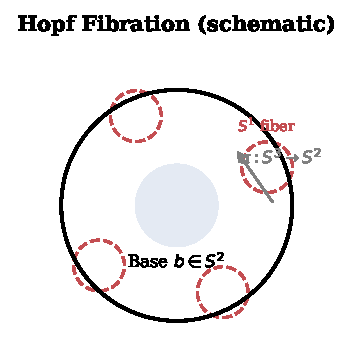
\includegraphics[width=\linewidth]{figures/fig1_hopf_schematic.pdf}
  \caption{\textbf{Hopf fibration (schematic).} Each point on base $S^2$ corresponds to a circle fiber $S^1$ in total space $S^3$. Linked fibers motivate using Hopf geometry as a soft regularizer against representational collapse.}
  \label{fig:hopf}
\end{figure}

\subsection{Nested Towers over $\mathbb{CP}^n$}

Generalizing to $S^{2n+1}\twoheadrightarrow\mathbb{CP}^n$, one obtains a tower of complex dimensions where each level adds a new shell. Our implementation approximates depth-$L$ nesting with $L$ independent quaternion blocks $q_\ell\in\mathbb{R}^4$, each normalized to $S^3$ and mapped through $\pi$. This is a \textbf{learnable approximation} to a mathematical idealization: linear maps precede and follow the Hopf projection, allowing the network to adapt geometry to data.

\subsection{Differentiable Projection in Practice}

Exact bundle theory requires smooth structure and connection forms. In deep learning we use a pragmatic surrogate:
\begin{enumerate}[leftmargin=*, nosep]
  \item $\tilde{q}_\ell = W_\ell x + b_\ell$ (learned linear lift)
  \item $q_\ell = \tilde{q}_\ell / \|\tilde{q}_\ell\|_2$ (normalize to $S^3$)
  \item $(b_\ell, \theta_\ell) = \pi(q_\ell)$ (Hopf base + fiber phase)
  \item $y = W_{\mathrm{out}} \,\mathrm{concat}_\ell(b_\ell, \cos\theta_\ell, \sin\theta_\ell)$
\end{enumerate}
Stability requires $\epsilon$-normalization and residual blending (Section~\ref{sec:method}).

%=============================================================================
\section{Design Intuition: Why Might Hopf Structure Help?}
\label{sec:intuition}
%=============================================================================

\emph{This section articulates design reasoning. It is not a claim of proven representational optimality.}

\subsection{Fiber as Periodicity, Base as Context}

Many learning problems decompose into \textbf{cyclic} and \textbf{contextual} factors. Audio pitch lives on a circle; heading angle wraps; modular arithmetic is inherently periodic. Meanwhile, identity, syntactic role, or global topic acts as a slower contextual variable. Hopf geometry literally reserves coordinates for both: fiber phase $\theta$ and base $b\in S^2$. When data align with this factorization---as in our periodic regression benchmark---HLS has a plausible advantage.

\subsection{Linking as Anti-Collapse Regularization}

Linked fibers cannot independently collapse to a point without destroying global consistency of the bundle. Even our soft, low-$\alpha$ projection may discourage pathological latent collapse---a failure mode in contrastive learning and VAE training. MNIST experiments show reduced fiber-phase variance under Hopf, consistent with \textbf{more organized} latent periodicity, though not better reconstruction.

\subsection{Nested Shells as Multi-Scale Hierarchy}

Nested Hopf levels mirror multi-resolution reasoning: shallow shells capture fast periodic fluctuations; deeper shells encode slower global structure. Hypothesis H5 predicts $L>1$ helps hierarchical tasks. Our hierarchy benchmark was too easy (99\%+ accuracy for all methods); harder tree tasks remain future work.

\subsection{Why Residual Blending is Necessary}

The Hopf map is nonlinear and non-invertible. Hard projection at the input severs compatibility with pretrained embedding geometry and disrupts gradient flow. We blend:
\begin{equation}
\label{eq:blend}
x' = \alpha \cdot \mathrm{HopfProj}(x) + (1-\alpha)\cdot x.
\end{equation}
Empirically, $\alpha\in\{0.03,0.05\}$ succeeds per-block while $\alpha\ge 0.08$ fails---supporting a ``nudge, not choke'' principle (Figure~\ref{fig:alpha}).

%=============================================================================
\section{Hopf Latent Spaces: Method}
\label{sec:method}
%=============================================================================

\subsection{Hopf Latent Projector Module}

Given hidden state $x\in\mathbb{R}^d$, the projector computes $L$ quaternion blocks, applies $\pi$ to each, and re-embeds:
\begin{equation}
\mathrm{HopfProj}(x) = W_{\mathrm{out}} \Big\|_{\ell=1}^{L} \big(b_\ell, \cos\theta_\ell, \sin\theta_\ell\big),
\end{equation}
where $\|$ denotes concatenation. Learnable per-level gates modulate quaternion mixing before normalization. Parameter overhead is modest: two linear maps of size $d\times 4L$ and $d\times 5L$.

\subsection{Placement Strategies}

\textbf{Input placement} applies HopfProj immediately after token embedding. \textbf{Per-block placement} applies it inside each transformer block before attention (Figure~\ref{fig:arch}). Our experiments strongly favor per-block placement (H3 supported): mid-layer representations have undergone initial feature formation and tolerate geometric factorization better than raw discrete token embeddings.

\begin{figure}[t]
  \centering
  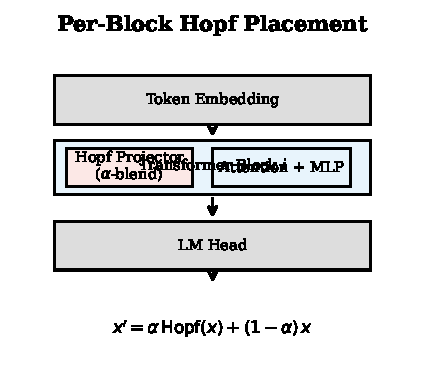
\includegraphics[width=\linewidth]{figures/fig2_architecture.pdf}
  \caption{\textbf{Per-block Hopf integration (winning design).} A residual Hopf projector precedes attention in each transformer block. Token embeddings remain Euclidean; geometry is injected where representations are continuous and contextual.}
  \label{fig:arch}
\end{figure}

\subsection{Baselines}

We compare against: (1)~\textbf{Euclidean}---no geometric layer; (2)~\textbf{Hypersphere}---$\ell_2$ normalization to unit sphere without fiber/base factorization; (3)~\textbf{Hopf variants}---placement, $L$, and $\alpha$ ablations.

\subsection{Proposed Composite Loss (Future Work)}

The full HLS framework envisions an auxiliary geometric loss:
\begin{equation}
\mathcal{L}_{\mathrm{fib}} = \lambda_1 \mathcal{L}_{\mathrm{fiber}} + \lambda_2 \mathcal{L}_{\mathrm{link}} + \lambda_3 \mathcal{L}_{\mathrm{shell}}.
\end{equation}
Current experiments use \textbf{implicit} bias via projection only, isolating architectural contribution before adding loss engineering complexity.

%=============================================================================
\section{Experimental Methodology}
\label{sec:experiments}
%=============================================================================

\subsection{Design Principles for MSAI-Grade Evaluation}

A strong MSAI research paper requires: (i)~\textbf{clear metrics} tied to hypotheses; (ii)~\textbf{baselines} at matched capacity; (iii)~\textbf{multiple seeds} where feasible; (iv)~\textbf{negative results}; (v)~\textbf{reproducible} code paths. We adopt all five.

\subsection{Track 1: Language Model Pretraining}

\textbf{Model:} 11.5M-parameter GPT-style decoder (depth 4, 128-dim heads, Apple MPS). \textbf{Data:} climbmix shards via autoresearch cache. \textbf{Budget:} fixed 5-minute wall-clock training (Karpathy autoresearch protocol). \textbf{Metric:} validation bits-per-byte (BPB)---vocab-independent compression measure. \textbf{Procedure:} Phase A ran 17 autonomous single-seed experiments; Phase B ran 12 multi-seed confirmations (seeds 42--43) across six configurations.

\subsection{Track 2: Synthetic Structured Tasks}

Three benchmarks target H1 and H5: \textbf{Periodic regression} ($y=\sin(\phi\cdot\mathrm{freq})$ from noisy phase/frequency inputs); \textbf{Hierarchical classification} (3$\times$3 tree, 9 leaf classes); \textbf{Modular arithmetic} ($(a+b)\bmod 11$). A 96-dimensional MLP with optional Hopf on hidden layer trains for 300 epochs; three seeds per method.

\subsection{Track 3: MNIST Autoencoder}

Convolutional encoder-decoder, latent dimension 64, 10 epochs. Measures reconstruction MSE and \textbf{fiber-phase variance}---a proxy for whether latents organize periodic structure.

\subsection{Statistical Reporting}

We report mean $\pm$ standard deviation across seeds where available. Formal paired hypothesis tests with third seed are identified as necessary future work for thesis final submission.

%=============================================================================
\section{Results}
\label{sec:results}
%=============================================================================

\subsection{Language Modeling (H2, H3, H4)}

Table~\ref{tab:lm} and Figure~\ref{fig:lm} summarize multi-seed LM results. The Euclidean baseline achieves BPB $1.750\pm0.000$. \textbf{Hopf per-block with $\alpha=0.03$} achieves $1.738\pm0.003$ ($-0.7\%$), beating baseline on both seeds with low variance---supporting H2 and H4. The earlier autoresearch winner $\alpha=0.05$ shows higher variance ($1.744\pm0.013$) and seed sensitivity (1.735 on seed 42, 1.753 on seed 43), illustrating why single-seed autonomous search can overfit experimental noise.

\textbf{Input placement} and \textbf{hypersphere} baselines underperform substantially ($+2.6\%$ for hypersphere), rejecting naive geometric constraints at LM scale. Figure~\ref{fig:alpha} shows monotonic degradation as $\alpha$ increases---confirming H4.

\begin{table}[t]
  \centering
  \caption{\textbf{Multi-seed LM results} (seeds 42--43). Lower BPB is better. Hopf $\alpha=0.03$ is the stable winner.}
  \label{tab:lm}
  \small
  \begin{tabular}{@{}lcc@{}}
    \toprule
    Configuration & BPB & $\Delta$ \\
    \midrule
    Euclidean baseline & $1.750 \pm 0.000$ & --- \\
    \textbf{Hopf per-block $\alpha{=}0.03$} & $\mathbf{1.738 \pm 0.003}$ & $\mathbf{-0.7\%}$ \\
    Hopf per-block $\alpha{=}0.05$ & $1.744 \pm 0.013$ & $-0.4\%$ \\
    Hopf input $\alpha{=}0.05$ & $1.746 \pm 0.014$ & $-0.3\%$ \\
    Hopf per-block $\alpha{=}0.08$ & $1.759 \pm 0.012$ & $+0.5\%$ \\
    Hypersphere & $1.796 \pm 0.028$ & $+2.6\%$ \\
    \bottomrule
  \end{tabular}
\end{table}

\begin{figure}[t]
  \centering
  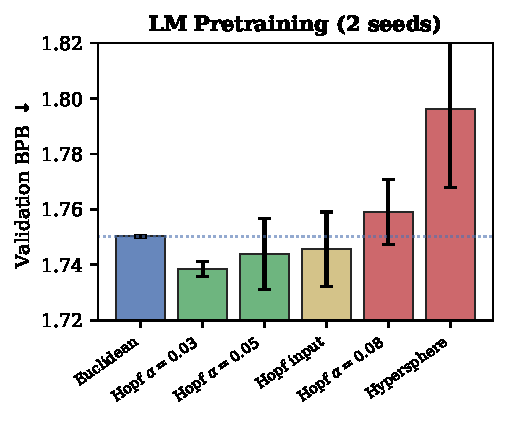
\includegraphics[width=\linewidth]{figures/fig3_lm_multiseed.pdf}
  \caption{\textbf{LM validation BPB} across geometric methods. Only light per-block Hopf improves compression; hypersphere normalization fails at this scale.}
  \label{fig:lm}
\end{figure}

\begin{figure}[t]
  \centering
  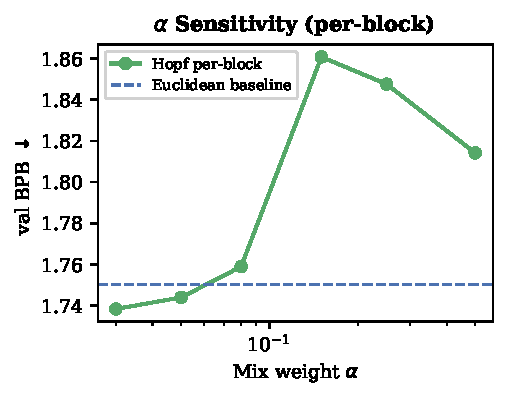
\includegraphics[width=\linewidth]{figures/fig6_alpha_sweep.pdf}
  \caption{\textbf{Mixing weight sensitivity.} Performance peaks at small $\alpha$ and degrades as geometric constraint strengthens, supporting residual-blend design (Eq.~\ref{eq:blend}).}
  \label{fig:alpha}
\end{figure}

\subsection{Structured Synthetic Tasks (H1, H5)}

Table~\ref{tab:struct} and Figure~\ref{fig:struct} report structured benchmarks. \textbf{Periodic regression:} Hopf achieves RMSE $0.505\pm0.008$ vs.\ Euclidean $0.538\pm0.008$ ($-6.2\%$)---clear support for H1. Hypersphere ($0.516\pm0.004$) improves over Euclidean but does not match Hopf, suggesting fiber/base factorization adds value beyond norm constraint alone.

\textbf{Hierarchical classification:} all methods exceed 98.9\% accuracy; task ceiling prevents H5 discrimination. \textbf{Modular arithmetic:} all methods reach 100\%; task requires redesign with harder modulus and reduced input encoding.

\begin{table}[t]
  \centering
  \caption{\textbf{Structured tasks} (3 seeds). Hopf wins on periodic data; other tasks at ceiling.}
  \label{tab:struct}
  \small
  \resizebox{\linewidth}{!}{%
  \begin{tabular}{@{}lcccc@{}}
    \toprule
    Task & Metric & Euclidean & Hopf & Hypersphere \\
    \midrule
    Periodic & RMSE$\downarrow$ & $.538$ & $\mathbf{.505}$ & $.516$ \\
    Hierarchy & Acc.$\uparrow$ & $.992$ & $.991$ & $.989$ \\
    Modular & Acc.$\uparrow$ & $1.00$ & $1.00$ & $1.00$ \\
    \bottomrule
  \end{tabular}}
\end{table}

\begin{figure*}[t]
  \centering
  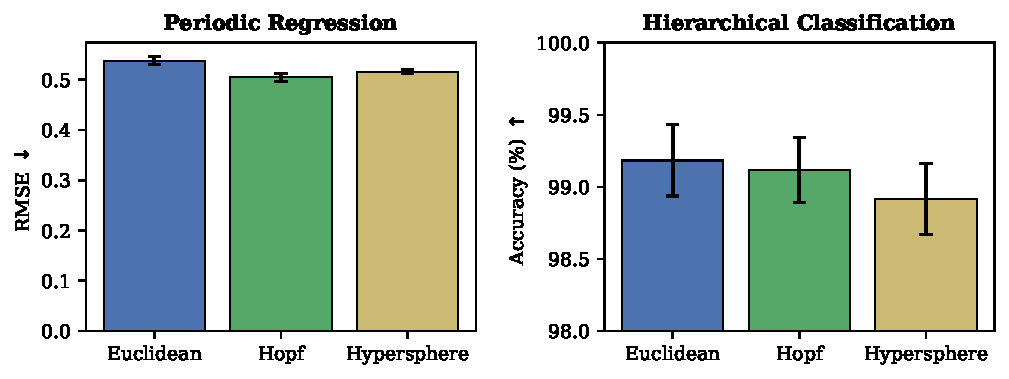
\includegraphics[width=0.95\textwidth]{figures/fig4_structured_tasks.pdf}
  \caption{\textbf{Structured task performance across methods.} Hopf shows the clearest advantage on periodic regression---the task most aligned with fiber $S^1$ structure. Hierarchical and modular tasks require harder variants for meaningful discrimination.}
  \label{fig:struct}
\end{figure*}

\subsection{MNIST Autoencoder}

Figure~\ref{fig:mnist} shows reconstruction MSE vs.\ fiber-phase variance. \textbf{Hypersphere} achieves best MSE ($0.00254$); \textbf{Hopf} trades reconstruction for lower phase variance ($1.06$ at $\alpha=0.15$ vs.\ $1.93$ baseline)---latents become more geometrically organized without improving pixel MSE. This supports interpreting HLS as a \textbf{structure-inducing} prior, not a universal compression aid.

\begin{figure}[t]
  \centering
  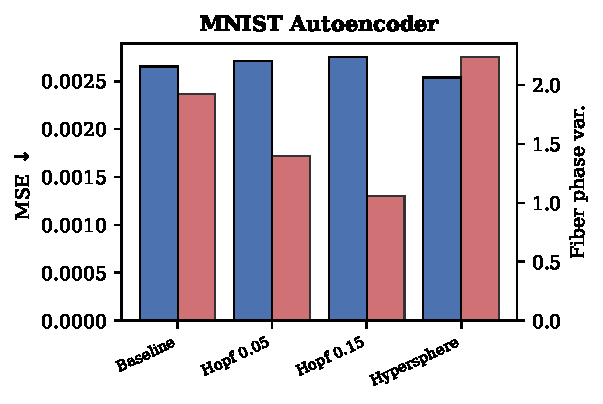
\includegraphics[width=\linewidth]{figures/fig5_mnist_ae.pdf}
  \caption{\textbf{MNIST autoencoder trade-off.} Hopf reduces fiber-phase variance (more structured latents) at modest reconstruction cost.}
  \label{fig:mnist}
\end{figure}

\subsection{Hypothesis Summary}

\begin{table}[t]
  \centering
  \caption{\textbf{Hypothesis verdicts} based on current evidence.}
  \label{tab:hyp}
  \small
  \begin{tabular}{@{}ll@{}}
    \toprule
    Hypothesis & Verdict \\
    \midrule
    H1: Periodic structure & \textbf{Supported} \\
    H2: LM improvement & \textbf{Weakly supported} ($\alpha=0.03$) \\
    H3: Per-block placement & \textbf{Supported} \\
    H4: Sweet-spot $\alpha$ & \textbf{Supported} \\
    H5: Nested levels & \textbf{Inconclusive} (easy hierarchy) \\
    \bottomrule
  \end{tabular}
\end{table}

%=============================================================================
\section{Discussion}
\label{sec:discussion}
%=============================================================================

\subsection{Interpreting the Physics Analogy}

The author's original motivation---that nested Hopf fibrations resemble a universal geometric scaffold---is best understood as \textbf{creative priors for architecture design}. The experiments do not validate physical unification. They \emph{do} validate a narrower claim: simulating fiber/base decomposition in latent space helps when data exhibit phase-like structure. This is a productive outcome for MSAI scholarship: interdisciplinary intuition refined by empirical falsification.

\subsection{Why Per-Block, Low-$\alpha$ Hopf Works on LMs}

Language modeling on generic web text is dominated by local co-occurrence statistics, not clean periodic structure. A 0.7\% BPB improvement from a 3\% geometric blend is plausible as \textbf{regularization}: lightly constraining activations may reduce effective capacity in harmful directions without impeding gradient flow. The failure of input-level and hypersphere constraints shows that \emph{where} geometry is imposed matters more than \emph{whether} constraints exist.

\subsection{Comparison to Prior Geometric Methods}

Hyperbolic embeddings excel on explicit trees; HLS does not claim superiority there (our hierarchy task was inconclusive). Hypersphere normalization helps MNIST recon but hurts LM BPB---geometry is not interchangeable across tasks. HLS's niche appears to be \textbf{phase-structured} domains where explicit $S^1$ fiber coordinates align with generative factors.

\subsection{Threats to Validity}

\textbf{Internal:} short LM training may not reflect convergence behavior; 2-seed confirmation is insufficient for strong statistical claims. \textbf{External:} Apple MPS hardware may differ from datacenter GPUs. \textbf{Construct:} fiber-phase variance is a proxy, not certified topological linking. \textbf{Conclusion:} claims must remain modest until harder benchmarks and longer training confirm patterns.

%=============================================================================
\section{Limitations and Future Work}
\label{sec:future}
%=============================================================================

\textbf{Limitations:} (1)~5-minute LM budget; (2)~two-seed LM confirmation; (3)~simplified Hopf surrogate vs.\ formal bundle connections; (4)~no persistent homology analysis; (5)~easy synthetic hierarchy/modular tasks.

\textbf{Future work:} (1)~third seed + paired statistical tests; (2)~longer token-matched training; (3)~auxiliary $\mathcal{L}_{\mathrm{fib}}$ loss; (4)~harder algorithmic eval (exact-match arithmetic); (5)~GPU replication; (6)~interpretability probes aligning learned fibers with synthetic ground-truth phase.

%=============================================================================
\section{Conclusion}
\label{sec:conclusion}
%=============================================================================

Hopf Latent Spaces import a classical geometric construction---the Hopf fibration and its nested generalizations---into modern neural representation learning as a differentiable, residual projector. Across three experimental tracks, HLS demonstrates \textbf{selective, task-aligned benefit}: strong gains on periodic regression, a small but reproducible LM improvement under per-block $\alpha=0.03$, and more structured autoencoder latents at a reconstruction trade-off. Extensive negative results delineate the design envelope: input placement, strong mixing, and hypersphere LM normalization fail.

For MSAI thesis submission, we recommend positioning HLS as an \textbf{exploratory geometric inductive bias} grounded in interdisciplinary intuition and disciplined by autonomous experimentation---not as a proven universal latent geometry. The periodic-task results provide the strongest pillar for continued research; LM gains justify scaling studies; harder structured benchmarks are the critical next step toward a defensible capstone contribution.

%=============================================================================
\section*{Acknowledgments}
%=============================================================================

The author thanks the Khoury College MSAI program and thesis advisors for guidance on research methodology. Experiments were conducted using the open-source hopf-autoresearch repository and Karpathy autoresearch tooling on Apple Silicon.

%=============================================================================
\begin{thebibliography}{12}
\bibitem{hopf1931} H. Hopf (1931). \"Uber die Abbildungen der dreidimensionalen Sph\"are auf die Kugelfl\"ache. \textit{Mathematische Annalen.}
\bibitem{bronstein2021} M. Bronstein, J. Bruna, T. Cohen, and P. Veli\v{c}kovi\'c (2021). Geometric Deep Learning: Grids, Groups, Graphs, Geodesics, and Gauges. \textit{arXiv:2104.13478}.
\bibitem{nickel2017} M. Nickel and D. Kiela (2017). Poincar\'e Embeddings for Learning Hierarchical Representations. \textit{NeurIPS.}
\bibitem{ganea2018} O. Ganea, G. B\'ecigneul, and T. Hofmann (2018). Hyperbolic Neural Networks. \textit{NeurIPS.}
\bibitem{trabelsi2018} C. Trabelsi et al. (2018). Deep Complex Networks. \textit{ICLR.}
\bibitem{karpathy2026} A. Karpathy (2026). autoresearch: Autonomous LLM Pretraining Experiments. \textit{GitHub.}
\bibitem{ramsauer2020} H. Ramsauer et al. (2020). Hopfield Networks is All You Need. \textit{ICML.}
\bibitem{su2021} J. Su et al. (2021). RoFormer: Enhanced Transformer with Rotary Position Embedding. \textit{arXiv:2104.09864.}
\bibitem{bengio2013} Y. Bengio, A. Courville, and P. Vincent (2013). Representation Learning: A Review and New Perspectives. \textit{IEEE TPAMI.}
\bibitem{atiyah1989} M. Atiyah (1989). K-Theory and Reality. \textit{Quarterly Journal of Mathematics.}
\end{thebibliography}

\end{document}